\chapter{Schoenflies}

\comm{Agregar: Toda variedad compacta con borde tiene entorno collar.

Las clausuras de las componentes del complemento cuando no son variedades se llaman crumpled cubes, y bing prueba que un crumpled $n$-cube siempre es un retracto de $R^n$, esto implica q son contractibles.

Puede pasar q las dos componentes sean crumpled cubes, x ejemplo agarras la esfera de alexander y le pones cuernos para el otro lado tb. también hay una prueba de q agarrar la esfera y hacerle el doubling queda $S^3$}

La idea de la prueba es empezar asumiendo que una de las componentes es una variedad $A$, y en ese caso encontrar un entorno de collar para $A$. Teniendo ese entorno uno se considera un disco $D_1$ qu eesté contenido en $\partial A\times [0,1]\subset A$. Tomamos $D_2=S^n-D_1$ y se cumple que $D_2\simeq \D^n$. La idea después es probar que el homeo $D_2\simeq \D^n$ se extiende a un homeo $A\simeq \D^n$, esta es la parte que lleva más trabajo, la meat and potato de la prueba.

\iffalse

\begin{teo}
    Sea $f:Q\to \s^n$ una función continua entre una $n$-célula $Q$ y $\s^n$ tal que el conjunto $X=\{x\in\s^n :\# f^{-1}(x)> 1\}$ es finito y $f^{-1}(X)$ está contenido en el interior de $Q$ y es finito.

    Entonces, si escribimos $\s^n - f(\mathring{Q})= D_1\sqcup D_2$, se tiene que $f(Q)=D_1\cup f(\partial Q)$ o $f(Q)=D_2\cup f(\partial Q)$
\end{teo}

\begin{dem}

    Llamamos $h=f|_{\mathring{Q}}$, $h$ es continua e inyectiva entre espacios métricos compactos, entonces es un homeo sobre su imagen. Como vimos antes en el teorema de separación de Jordan-Brouwer, $h(\mathring{Q})$ separa $\s^n$ en dos componentes conexas (y estas componentes son bolas homológicas).

    En principio tenemos dos opciones:

    \begin{itemize}
        \item $f(Q)\subset f(\partial Q)$
        \item $f(\mathring{Q})$ intersecta $D_1\sqcup D_2$
    \end{itemize}
    
    Supongamos $f(Q)\subset f(\partial Q)$. En ese caso podríamos considerar la composición $h^{-1}\circ f$. Esta sería una función continua que fija $\partial Q$ y manda $Q$ en $\partial Q$, esto es absurdo. 
    
    \comm{escribir esto con más detalle?}

    Obtuvimos entonces que $f(Q)$ intersecta por lo menos a una de las regiones $D_1$, $D_2$. Llamemos $D$ a una tal que $f(Q)\cap D\neq\varnothing$.

    Como $f^{-1}(X)\cap\partial Q=\varnothing$, se cumple que $f$ es inyectiva en $\partial Q$. Además $f^{-1}(f(\partial Q))=\partial Q$. 

    $\partial{Q}$ no separa $Q$, $f(\partial{Q})$ separa $\s^n$, entonces $f(Q)\subset\overline{D}$. \comm{escribir mejor}

    Si la inclusión es estricta, 


    % $\int{Q}$ es conexo, entonces $f(\int{Q})$ es conexo. Además $f(\int{Q})\cap D\neq\varnothing$, entonces $f(\int{Q})\subset D$. Por lo tanto $f(Q)=D\cup f(\partial Q)$.%    

\end{dem}

\fi

%\comm{ahora una prueba como la gente aver}

Idea de la prueba: Dado un encaje $\phi:\s^{n-1}\to\s^n$, consideramos $D$ la clausura de una componente de $\s^n - \phi(\s^{n-1})$. Queremos probar que si $D$ es una variedad, entonces $D\simeq \D^n$.

Si $D$ es una variedad con borde, el borde tiene un entorno homeomorfo a $\s^{n-1}\times [0,1]$ en $D$. Llamamos $\hat{\phi}:\s^{n-1}\times [0,1]\to\s^n$ al encaje, que es una extensión de $\phi$.

Sean $X, Y$ las dos componentes de $\s^n-\hat{\phi}(\s^{n-1}\times [0,1])$ tal que $X\subset D$. Vamos a ver que existe un mapa sobreyectivo $f:\s^n\to\s^n$ tal que manda $X$, $Y$ en dos puntos distintos $x$, $y$, y es inyectiva en $\s^n-X\cup Y$. Una vez tenemos eso, restringiendo $f$ a $D$ tenemos como imagen un disco $\D\subset\s^n$.

La clave para esto es probar que bajo estas hipótesis $D$ cumple $D\simeq D/X$. Más específicamente, $D$ va a ser un $\textbf{conjunto celular}$.

\begin{df}
    Un subconjunto $X$ de una $n$-variedad es $\textbf{celular}$ si para todo abierto $U$ que contiene a $X$ existe una familia de conjuntos $\{D_i,i\in\N\}$ tales que 
    
    \begin{itemize}
        \item $X=\cap_{i=1}^\infty D_i$
        \item $D_i\simeq\D$, $D_i\subset U$ para todo $i\in\N$
        \item Los $D_i$ están encajados: $D_{i+1}\subset\mathring{D_i}$
    \end{itemize}
\end{df}

\begin{obs}
    Los $D_i$ son compactos, como la variedad es Hausdorff, entonces son cerrados. Por lo tanto $X$ necesariamente es cerrado.
\end{obs}

\begin{df}

    Sea $M$ una $n$-variedad compacta con borde, $X_1,\dots,X_k$ subconjuntos cerrados y disjuntos dos a dos. Llamamos $\textbf{colapsar}$ $X_1,\dots ,X_k$ en $M$ a considerar el espacio cociente $M'=M/ \sim $ dado por $x\sim x'\iff x,x'\in X_i$ para algún $i\in\{1,\dots,k\}$.

\end{df}

Lo interesante de los conjuntos celulares es que al colapsarlos obtenemos una variedad homeomorfa a la que teníamos originalmente.

\begin{lema}
    Sea $M$ una $n$-variedad compacta con borde, $X$ subconjunto celular de $\mathring{M}$. Entonces el espacio $M'$ obtenido de colapsar $X$ es homeomorfo a $M$.
\end{lema}

\begin{dem}
    Tenemos $X=\bigcap\limits^{\infty} D_i$, con $D_i$ discos encajados como en la definición. Construyamos un mapa sobreyectivo $f:M\to M$ tal que $f|_{M-X}$ es inyectiva y $f(X)=x_0$ para algún $x_0\in M$. Este mapa va a ser el límite de una sucesión de homeos que construimos inductivamente, empezando por $f_1:= \text{Id}$.

    Para definir $f_{k+1}$, vamos a asumir que ya tenemos definido un homeo $f_k$. Lo modificamos de la siguiente manera:

    Vamos a elegir un homeomorfismo auxiliar $\hat{g}_{k+1}:f_k(D_k)\to f_k(D_k)$ tal que 
    
    \begin{itemize}
        \item $\hat{g}_{k+1}|_{\partial(f_k(D_k))}\equiv Id$
        \item $\diam\big(\hat{g}_{k+1}(f_k(D_{k+1}))\big)<\frac{1}{k+1}$
    \end{itemize}

    \comm{para el primer punto, entiendo que se está usando que el mapping class group de $\D^n$ es trivial, para poder "isotopar" $f_k|_{\partial D_k}$ a $\text{Id}$.}
    
    Una vez tenemos eso, lo extendemos a un homeo $g_{k+1}:M\to M$ como $g_{k+1}\equiv \text{Id}$ afuera de $f_k(D_k)$. Definimos $f_{k+1}:= g_{k+1}\circ f_k$.
    
%    Por ser un homeo, $f_k$ va a cumplir:

%    \begin{itemize}
%        \item $f_k(D_k)\simeq f_k(D_{k+1})\simeq\D^n$
%        \item $f_k(D_{k+1})\subset\mathring{f(D_k)}$
%    \end{itemize}

    Ahora hay que verificar que la familia de funciones $\{f_k\}$ converge punto a punto. Veamos que la sucesión $f_k(p)$ converge para todo $p\in M$. Para esto separamos en los casos $p\in X$, $p\in M-X$.

    Veamos el caso $p\in X$. Se tiene $f_k(p)\in f_k(D_k)$ para todo $k\in\N$. Por construcción, las $f_k$ cumplen 
    
    \begin{itemize}
    \item $f_1(D_1)\supset f_2(D_2)\supset f_3(D_3)\supset\dots$
    \item $\lim\limits_{k\to\infty}\text{diam}(D_k)=0$
    \end{itemize}
    Por lo tanto, la intersección $\bigcap\limits^\infty f_k(D_k)$ consiste de un único punto $x_0$, y se cumple que $\lim\limits_{k\to\infty}f_k(p)=x_0$.

    Tomemos ahora $p\in M-X$. Como los $D_k$ están encajados y $p\not\in\cap_{k=1}^\infty D_k$, existe un $K\in\N$ tal que $p\not\in D_k$ para todo $k\geq K$. Por lo tanto, la sucesión $f_k(p)$ es constante a partir de $K$.

    Con esto tenemos que las $f_k$ convergen puntualmente, llamamos $f$ al límite.

    Sabemos que $f$ es continua por definición, y que $f^{-1}(x_0)=X$. Verifiquemos que $f$ es inyectiva en $M-X$ y sobreyectiva.

    Para probar que $f$ es sobreyectiva, vamos a ver que alcanza todo elemento de $M$. Ya sabemos que $f(X)=\{x_0\}$, entonces basta verificar que un punto arbitrario $x\in M-\{x_0\}$ está en la imagen de $f$. Efectivamente, si $x\in M-\{x_0\}$ entonces $x\not\in \cap^\infty_{k=1} f_k(D_k)$, y por lo tanto a partir de un $K\in\N$ se tiene $x\not\in f_K(D_K)$, entonces $f_K^{-1}(x)\cap D_K=\varnothing$. Luego la sucesión $f_k(x)$ es constante a partir de $K$, y se cumple que $f(f^{-1}_K(x))=f_K(f^{-1}_K(x))=x$, por lo tanto $x$ está en la imagen de $f$.

    Ahora veamos que $f$ es inyectiva en $M-X$. Para eso tomamos dos puntos $x\neq y\in M-X$. Como no están en $X$, las sucesiones $f_k(x), f_k(y)$ son eventualmente constantes, y por lo tanto podemos encontrar un $K\in\N$ tal que $f(x) = f_K(x)$, $f(y) = f_K(y)$. Como $f_K$ es un homeo y $x\neq y$, entonces $f(x)\neq f(y)$.

    Con esto tenemos que $f:M\to M$ baja al cociente como una biyección continua, que además va a ser un homeo porque va de un espacio compacto a uno Hausdorff. $\square$
\end{dem}

Inductivamente obtenemos el mismo resultado para un espacio con finitos conjuntos celulares disjuntos dos a dos.

\begin{cor}
Sea $M$ una $n$-variedad compacta con borde, sean $X_1,\dots,X_n$ subconjuntos celulares de $\mathring{M}$ disjuntos dos a dos. Entonces el espacio $M'$ obtenido al colapsar los $X_i$ es homeomorfo a $M$.
\end{cor}

\begin{dem}
    Lo único que nos falta observar para usar inductivamente el lema anterior es que dados dos conjuntos celulares disjuntos $X_1$ y $X_2$, el conjunto $X_2$ sigue siendo celular en $M/\sim$ al colapsar $X_1$.

    En efecto, esto se cumple por definición. El complemento de un punto en $M/\sim$ es abierto, por lo tanto nos podemos tomar un entorno abierto del conjunto $X_2$. 
    
    \comm{terminar de escribir esto, creo q tengo q usar algun tipo de regularidad para decir que tengo el entorno abierto del conjunto. con eso ya sale que es celular en el colapsado.}
\end{dem}

Para poder usar esta propiedad tan útil sobre los conjuntos celulares, va a ser necesario un criterio que nos permita identificarlos.

\begin{lema}
    Sean $X_1,\dots, X_m\subset\mathring{\D}^n$ cerrados disjuntos. Sea $M/_{\sim}$ el espacio obtenido al colapsar $X_1,\dots, X_m$ y sea $\pi:M\to M/_{\sim}$ la proyección.
\end{lema}

\begin{lema}
    Sea $f:\D^n\to \s^n$ continua, sea $M\subset \D^n$ tal que $f$ es inyectiva en $\D^n - M$ y $M=f^{-1}(x_0)$ para algún $x_0\in\s^n$. Entonces, $M$ es un conjunto celular en $\D^n$
\end{lema}

\begin{lema}
    Sea $S\subset \s^n$ una $(n-1)$-esfera encajada en $\s^n$, sea $D$ una de las componentes conexas de $\s^n-S$. Sea $f:\overline{D}\to R\simeq \D^n$ continua, tal que es inyectiva en $\overline{D}-M$, siendo $M$ un conjunto celular. Entonces, $\overline{D}\simeq\D^n$.
\end{lema}

\comm{cuando digo "colapsar $X_1,\dots,X_m$", se Asobreentiende que es colapsarlos a puntos distintos, no?}


\iffalse

\begin{teo}
    Invariancia del dominio:

    $U$ abierto de $\R^n$, $h:U\to\R^n$ continua e inyectiva, entonces $h(U)$ es abierto de $\R^n$.
\end{teo}


\begin{dem}

    Vemos $S^n$ como la compactificación de $R^n$, queremos probar que $h(U)$ es abierto en $S^n$.

    Sea $x\in U$, entonces $x$ es centro de un disco $D$ de dimensión $n$ contenido en $U$.

    Probemos que $h(D-\partial D)$ es un abierto de $\S^n$.

    $h$ continua e inyectiva, entonces $h|_{\partial D}$, $h|_{D}$ son encajes.

    Por el teorema de la sección anterior \comm{insertar bien la referencia} tenemos que $\tilde{H}_0(\s^n - h(\partial D))=\Z$, es decir, $H_0(\s^n - h(\partial D))=\Z\oplus\Z$. O sea, $\s^n - h(\partial D)$ está conformado por dos componentes conexas por caminos que son disjuntas entre sí. 
    
    Estas componentes van a ser $\s^n-h(D)$ y $h(D-\partial D)$. Para asegurarnos, tenemos que comprobar que las dos son conexas por caminos. Como $D-\partial D$ es conexo por caminos, entonces $h(D-\partial D)$ también.
    
    Ahora, el mismo teorema nos dice que $\tilde{H}_i(\s^n - h(D))=0\fall i\in\N$, por lo tanto $H_0(\s^n - h(\partial D))=\Z$ y entonces $\s^n - h(\partial D)$ es conexo por caminos.

    Para la conclusión del teorema, basta observar dos cosas. Primero, que para conjuntos abiertos las componentes conexas siempre son conexas por caminos.
    
    Segundo, que si un espacio se descompone en finitas componentes conexas, entonces las componentes son abiertas.
    
    Como $\s^n-h(\partial D) = \s^n-h(D) \sqcup h(D-\partial D) $ es abierto, entonces sus dos componentes conexas son abiertos de $\s^n-h(\partial D)$ conexos por caminos, y por lo tanto son abiertos de $\s^n$.

    Obtuvimos entonces que $h(D-\partial D)$ es abierto de $\s^n$.
\end{dem}

Con esto tenemos un resultado para variedades topológicas:

\begin{cor}

    Sean $M$, $N$ $n$-variedades con $M$ compacta, $N$ conexa. Entonces, si $h:M\to N$ es un encaje, necesariamente es un homeomorfismo.

\end{cor}

\begin{dem}

    Veamos que $h(M)$ es abierto y cerrado en $N$. 

    Por el teorema de invariancia del dominio, tenemos que $h(M)$ es abierto en $N$.
    
    Como $M$ es compacto y $f$ un encaje, entonces $h(M)$ es compacto. Como $N$ es hausdorff, entonces $h(M)$ es cerrado.
    
    Por lo tanto $h(M)=N$ y entonces $h:M\to N$ es un homeo.

\end{dem}

\begin{figure}
    	\centering
    	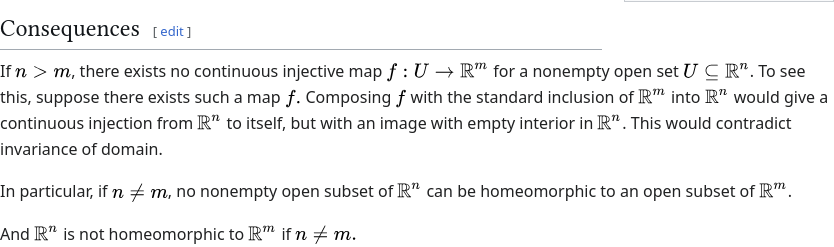
\includegraphics[width=0.75\linewidth]{img mono/schoenflies/inv dominio.png}
    	\caption{agregar esto}
\end{figure}

Podemos usar la invariancia del dominio para probar lo siguiente:

\begin{lema}
    Sea $M$ una $n$-variedad conexa con $n<1$, $P\subset M$ un conjunto finito, entonces $M-P$ es conexo.
\end{lema}

\comm{esta prueba es de las notas de Nikil Sahoo}

\begin{dem}
    Primero comenzamos observando que como nuestros espacios son Hausdorff, entonces los singleton $\{p\}$ son conjuntos cerrados. Por esta razón, los complementos de finitos puntos son subconjuntos abiertos de $M$, y por lo tanto son $n$-variedades.

    Por lo tanto, es suficiente probar el lema para $P=\{p\}$ un singleton. Veamos eso.

    Supongamos por absurdo que $M-\{p\}$ no es conexo, es decir, tenemos $U, V$ dos abiertos de $M-\{p\}$ tales que $M-\{p\}=U\sqcup V$. Estos también van a ser abiertos de $M$.

    \duda{por que son abiertos de M necesariamente?}

    Tomamos un entorno $U_p$ de $p$ en $M$ homeomorfo a $\D^n$, entonces $U_p - \{p\}$ es conexo, y por lo tanto está contenido en $U$ o en $V$. Supongamos que está en $U$, en ese caso $U_p-\{p\}\subset U$, y $U_p\cup U = U\cup\{p\}$, como ambos $U_p$ y $U$ son abiertos de $M$. Entonces $U\cup \{p\}$ es abierto en $M$ y obtenemos una descomposición de $M$ como dos abiertos disjuntos $(U\cup\{p\})\sqcup V$. Esto es absurdo ya que habíamos asumido $M$ conexa.
\end{dem}

\comm{leer https://mathoverflow.net/questions/29737/understand-cech-cohomology}

\fi